\documentclass{article}

\usepackage[margin=1in]{geometry}
\usepackage{listings}
\usepackage{color}
\usepackage{graphicx}
\usepackage{float}

\title{Lab 3: Interrupt Handling}
\date{October 17, 2017}
\author{Matthew Friedman 861151348\\Souradeep Bhattacharya 861105938\\EE128 Section: 021}

\definecolor{dkgreen}{rgb}{0,0.6,0}
\definecolor{gray}{rgb}{0.5,0.5,0.5}
\definecolor{mauve}{rgb}{0.58,0,0.82}

\lstset{frame=tb,
	language=C,
	aboveskip=3mm,
	belowskip=3mm,
	showstringspaces=false,
	columns=flexible,
	basicstyle={\small\ttfamily},
	numbers=none,
	numberstyle=\tiny\color{gray},
	keywordstyle=\color{blue},
	commentstyle=\color{dkgreen},
	stringstyle=\color{mauve},
	breaklines=true,
	breakatwhitespace=true,
	tabsize=4
}
\begin{document}
	\maketitle
	
	\section*{Abstract}
	\par
	The objective of this lab is to become familiar with interrupt-handling techniques for the 9S12DG256 microcontroller, and to improve skills on designing and debugging microcontroller based systems. In this lab we used the $\overline{IRQ}$ pin to generate interrupts. This pin was connected to an external clock signal and caused our hex counter to count up or down depending on the state of two switches.
	\section*{Experiment System Specification}
	\par
	We will design a "clock-tick" circuit which will drive a decimal 7-segment display. For every clock tick received the decimal point should pulse on and off. The display will be a two decade (0-99) 7-segment. The operation of the counter will be dictated by two switches:
	\begin{itemize}
		\item CNT HLD: 0 for normal operation, 1 for hold.
		\item CNT DIR: 0 for upward counting, and 1 for downward.
		\item The counter will wrap around if the end is reached.
	\end{itemize}
	\section*{Block Diagram and Hardware Design}
	\begin{figure}[H]
		\centering
		\includegraphics[width=1\textwidth]{Block_Diagram}
	\end{figure}

	\section*{Detailed Schematic Diagram}
		\begin{figure}[H]
		\centering
		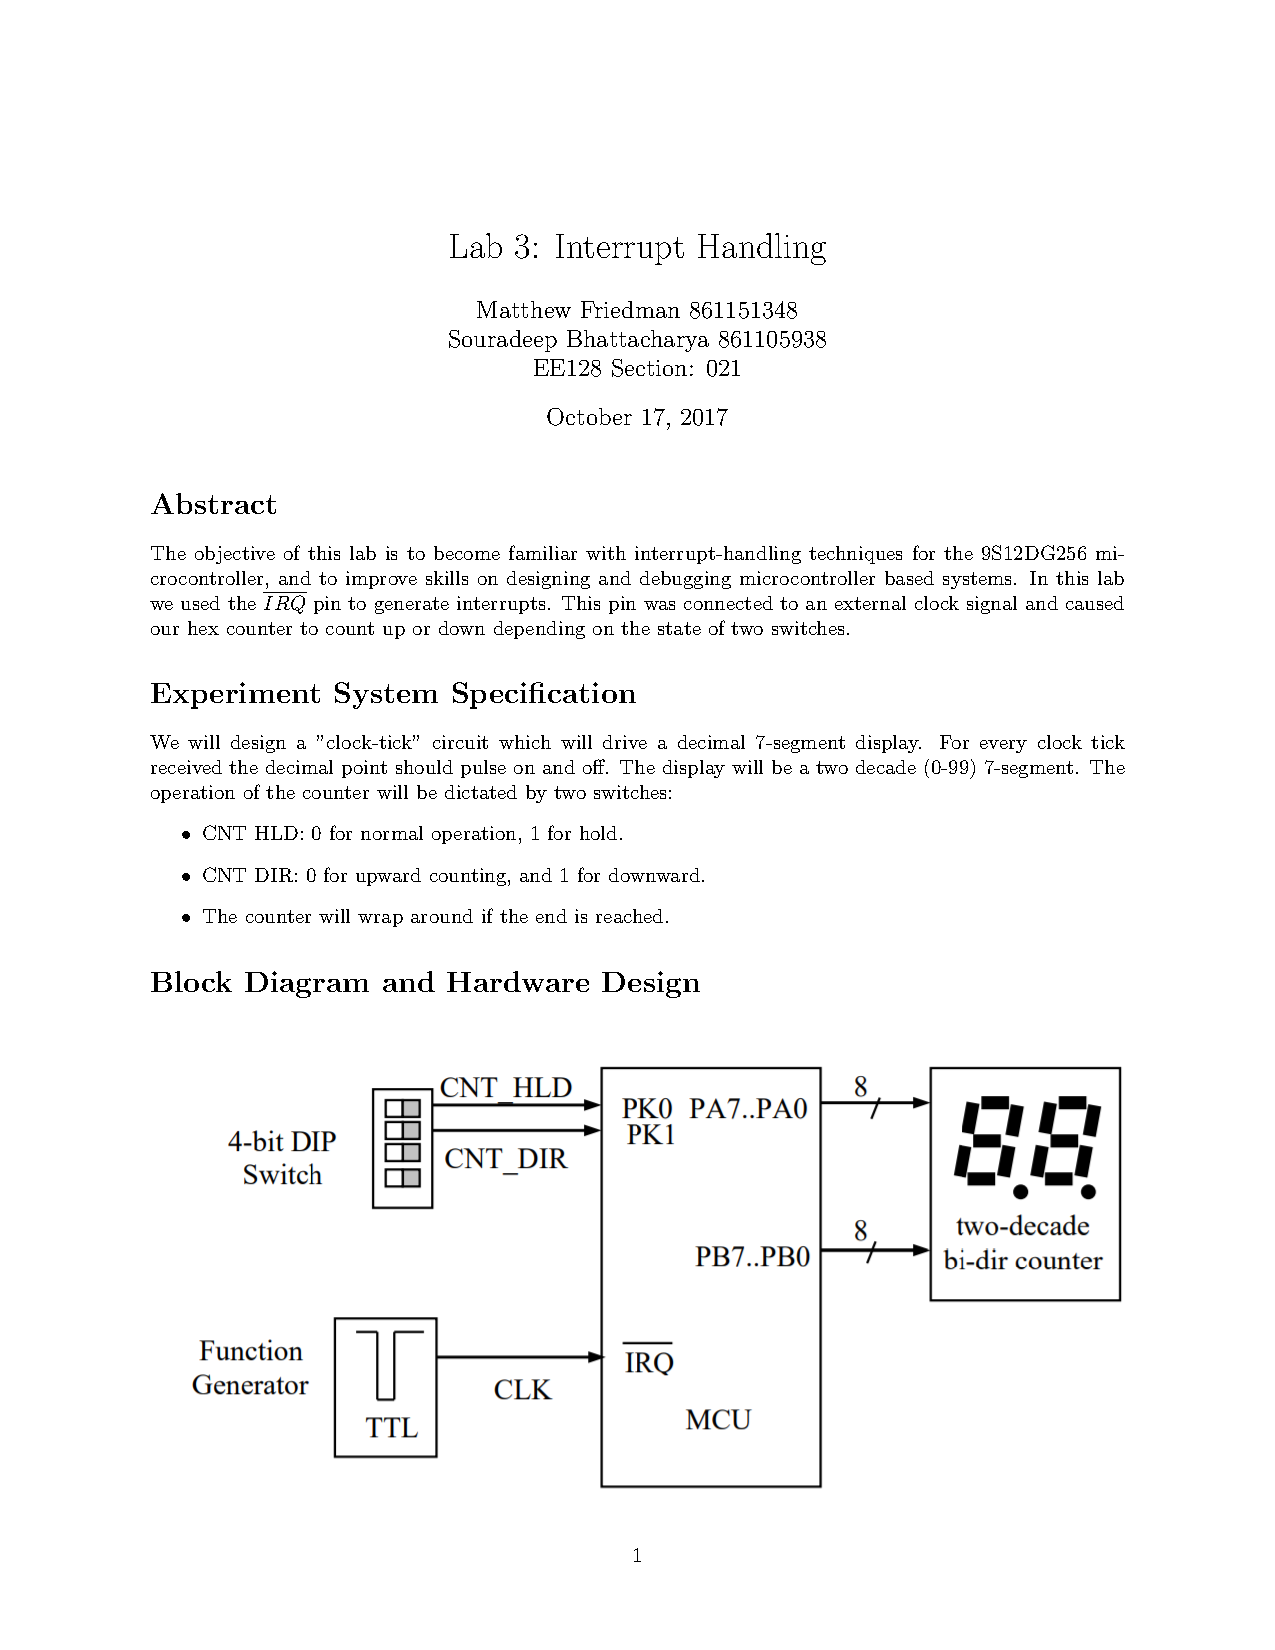
\includegraphics[width=1\textwidth]{Lab3}
	\end{figure}
	\section*{High level Description of Software}
	The programming will consist of two major sections:
	\begin{itemize}
		\item Update and display the clock tick
		\item Update and display the counter based on the switches.
	\end{itemize}
	The counter will wrap around when it reaches either end (0 or 99).
	\subsection*{Control Program}
	\paragraph{Configuration and Initialization}
	This part of the program sets up the ports, configures the interrupts, and initializes the counter.
	\paragraph{Interrupt Service Routine (ISR)}
	This portion of the program implements the following operations:
	\begin{itemize}
		\item Turn the LED on and off
		\item Update the two decade bi-directional counter
	\end{itemize}
	The ISR should implement the following pseudo-code:
	\begin{lstlisting}
	Let counter be a static variable initialized to 0;
	__interrupt void IRQ_ISR(void)
	{
		Update the clock tick and its display;
		Read Port K;
		
		if (CNT_HLD is 1) return; /* rotate hold */
		
		if (CNT_DIR is 1) /* rotate left */
			Count Down -- wrap around if end is reached;
		else
			Count Up – wrap around if end is reached;
		
		Update counter displays;
	}
	\end{lstlisting}
	\paragraph{Main Program}
	The main program after initialization should do nothing. But the main code should resemble the following:
	\begin{lstlisting}
	void main (void)
	{
		Configure Port A and B to be 8-bit output ports;
		Enable IRQ interrupts;
		for (;;){}
	}
	\end{lstlisting}
	\section*{Program Listing}
	\subsection*{C Code}
	\begin{lstlisting}
	#include <hidef.h>      /* common defines and macros */
	#include <mc9s12dg256.h>
	
	//declare globals
	unsigned char decoder[10] = {0x7E, 0x30, 0x6D, 0x79, 0x33, 0x5B, 0x5F, 0x70, 0x7F, 0x7B};
	char count = 0;
	char cnt_hold = 0;
	char cnt_dir = 0;
	
	//ISR definition
	interrupt void IRQ_ISR(void) 
	{
		//set variables by reading from PORTA
		cnt_hold = PORTK & 0x01;
		cnt_dir = PORTK & 0x02;
	
		if(cnt_hold == 0)     //cnt_hold = 0, so normal operation
		{
			if(cnt_dir)         //cnt_dir = 1 so dec
			{
					count--;
					if(count < 0) 
					{
						count = 99;      //roll over and start from the top
					} 
			} 
			else                //cnt_dir = 0 so inc
			{
				count++;
				if(count > 99) 
				{
					count = 0;      //roll over and start from bottom
				}
			}
		}
	
		//set 7-seg to value    
		PORTA = decoder[count/10] | ((PORTA & 0x80) ^ 0x80);
		PORTB = decoder[count%10] | ((PORTB & 0x80) ^ 0x80);
	}
	//init ISR function
	typedef void(*near tIsrFunc)(void);
	//setup ISR start address
	const tIsrFunc _vect @ 0x3E72 = IRQ_ISR;
	
	
	void main(void) 
	{  
		//setup ports  
		DDRB = 0xFF; //set port to output for 7-seg
		DDRE = 0x00; //set port to input for interrupt PORTE1
		DDRK = 0x00; //set port to input for dip switches
		DDRA = 0xFF; //set port to output for 7-seg
	
		//change settings for interrupt
		PORTE = 0x02;
		INTCR = 0xC0;
	
		EnableInterrupts;
	
		//init both 7segs
		PORTB = decoder[0];
		PORTA = decoder[0];
	
	
		while(1) 
		{
		}
	}
	
	\end{lstlisting}
	\subsection*{Project PRM}
	\begin{lstlisting}
	NAMES END
	SECTIONS
		MY_RAM = READ_WRITE 0x1000 TO 0x1FFF; /* 4095 bytes of data */
		MY_PSEUDO_ROM = READ_ONLY 0x2000 TO 0x3FFF; /* 8191 bytes of code */
	END
	
	PLACEMENT
		_PRESTART,
		STARTUP,
		ROM_VAR,
		STRINGS,
		DEFAULT_ROM, NON_BANKED,
		COPY INTO MY_PSEUDO_ROM;
		DEFAULT_RAM INTO MY_RAM;
	END
	
	STACKSIZE 0x100
	\end{lstlisting}
	
	\section*{Technical Problems}
	\paragraph*{Program wasn't working} We just hit the make button several times and it started working again.
	\paragraph*{Program wouldn't load} We had left the function generator output on and it would not load the program. We just had to turn off the output and reload it.
	\section*{Question Answers}
	\begin{enumerate}
		\item Based off of our image below our difference in falling edge is below 200 mS.
		\begin{figure}[H]
			\centering
			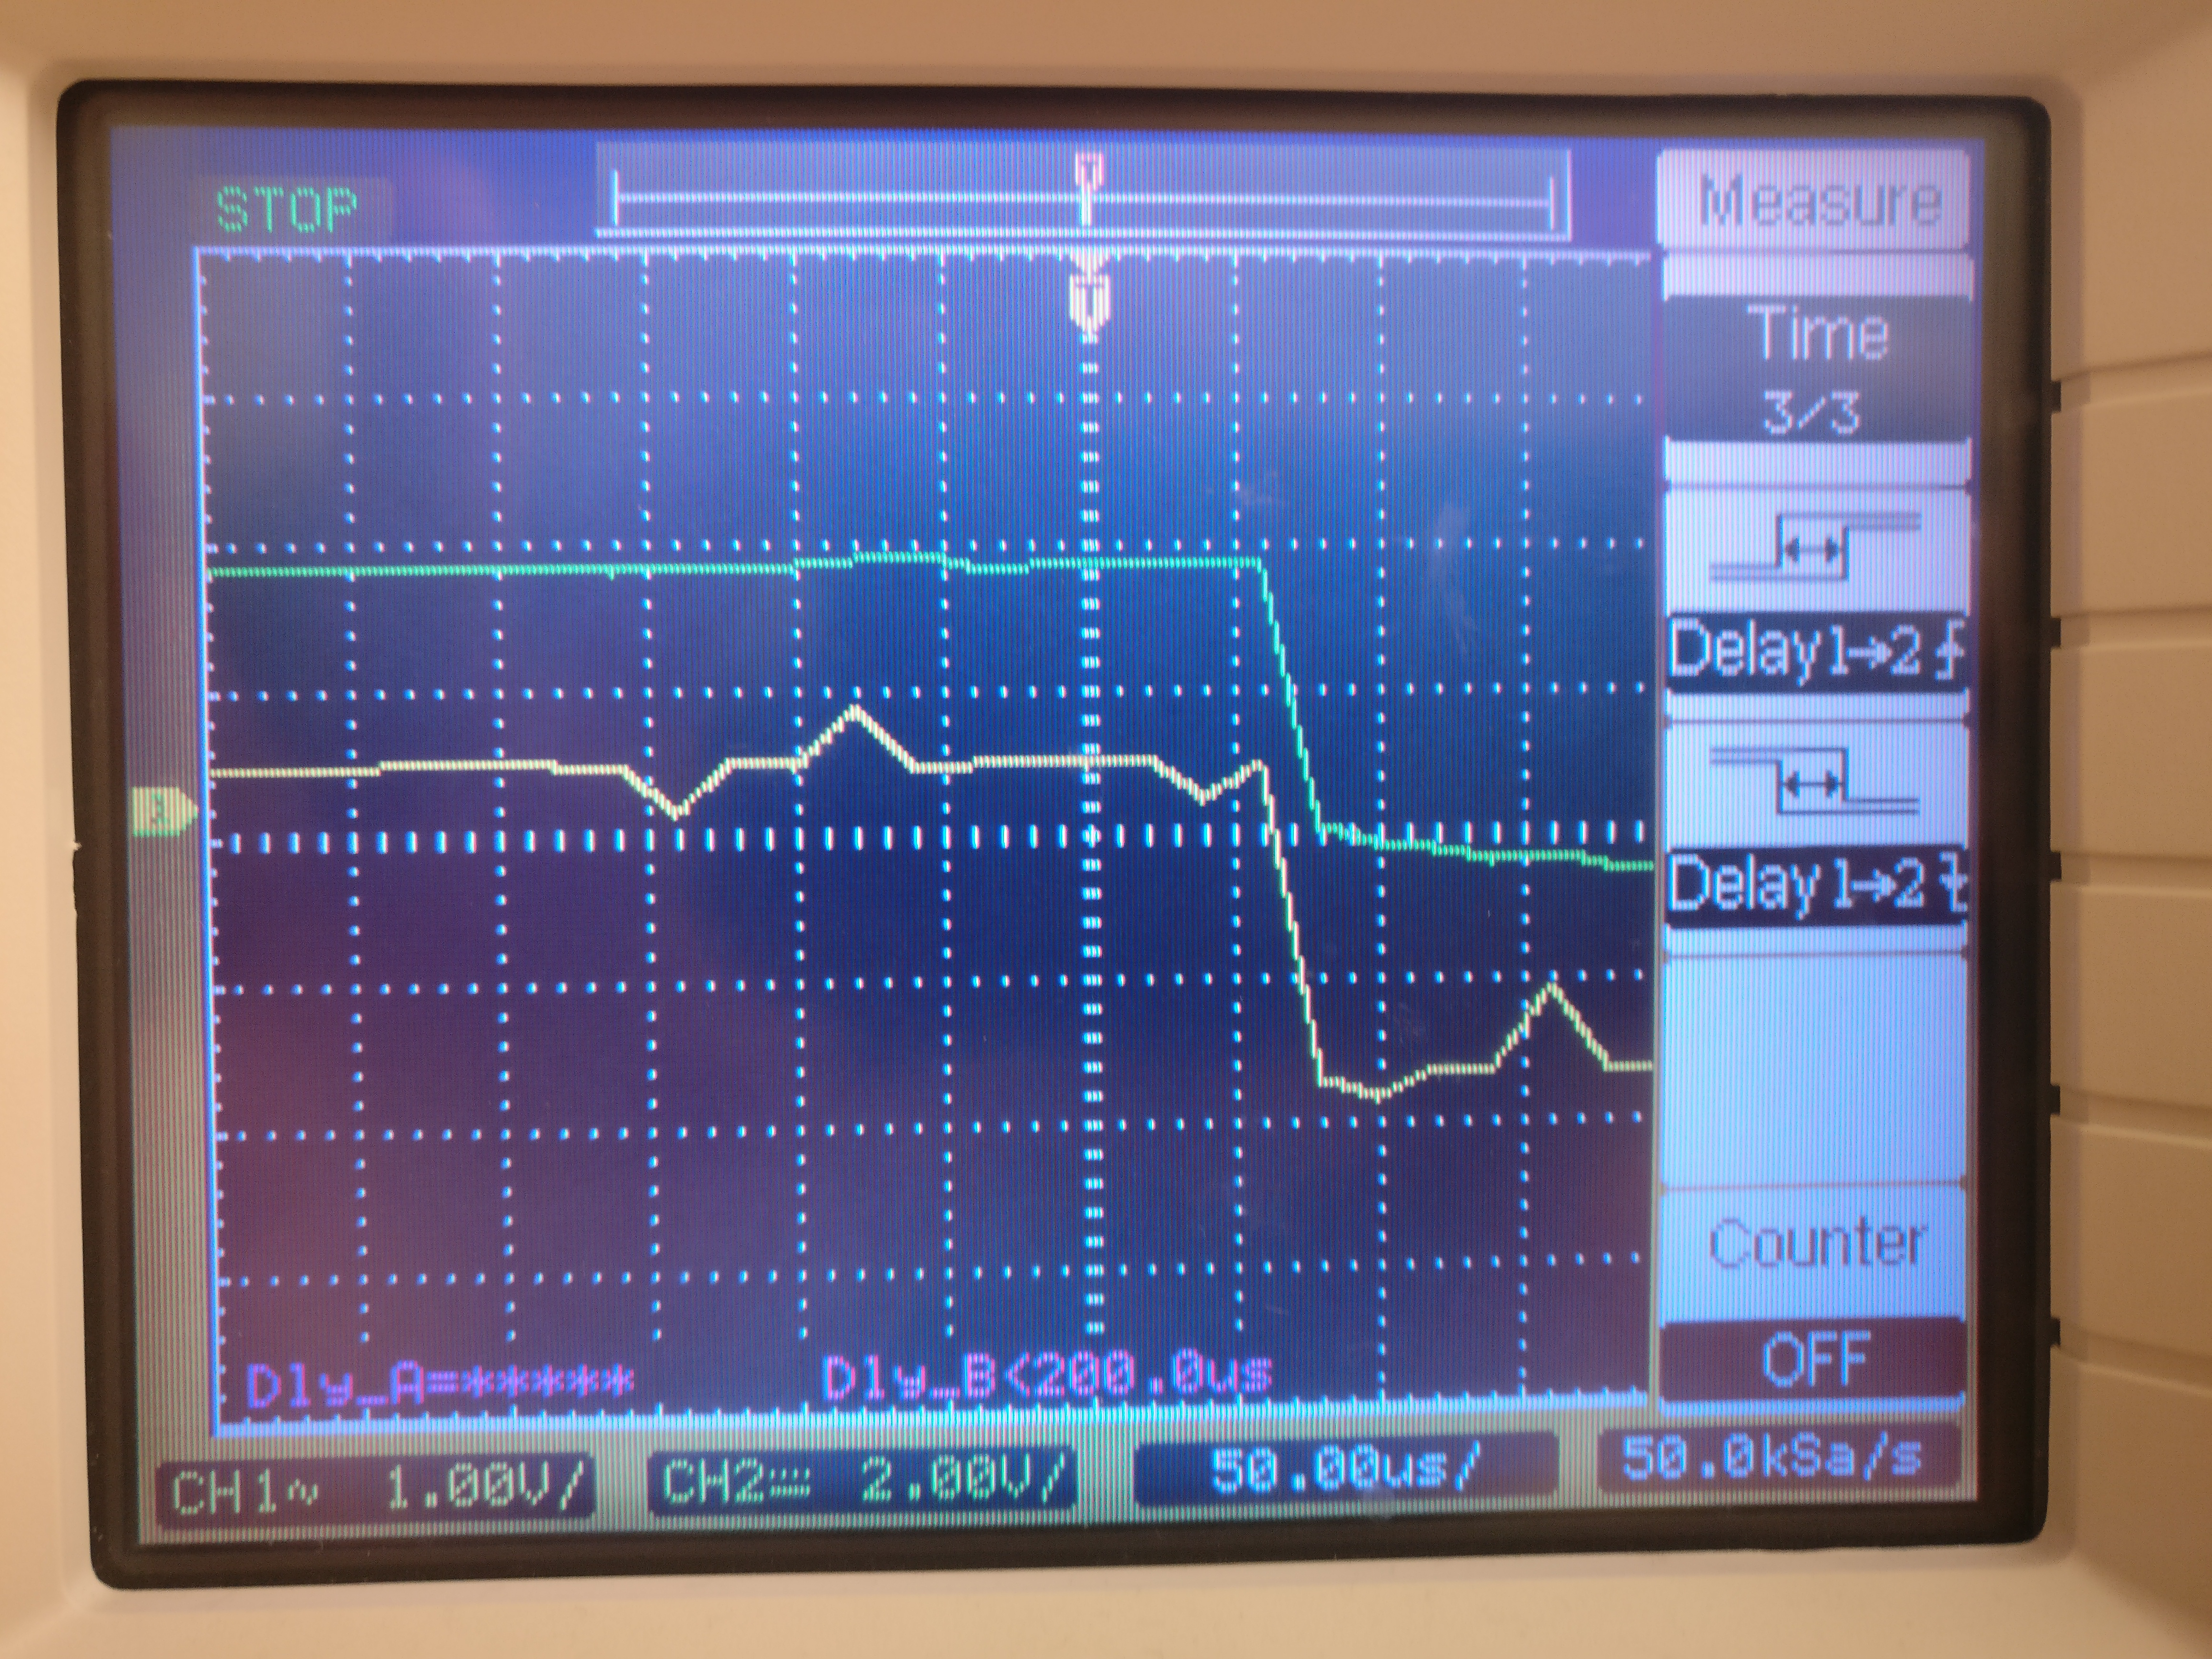
\includegraphics[width=1\textwidth]{Q1}
		\end{figure}
		\item Based off of our estimate our max clock frequency is 5KHz.
		\item We would need to use an ADC to convert the voltage level into a digital value. We would also need to change the interrupt to be something other than the IRQ pin, maybe if the external ADC used a SPI we would use the SPI interrupt.
	\end{enumerate}
	\section*{Conclusion}
	\par
	In this lab we learned how to create a Interrupt Service Routine(ISR). We used this ISR to create a bi-directional timer. Other then the listed technical difficulties we had no other major problems.
\end{document}